\documentclass[a5paper]{article}
\usepackage[a5paper, top=8mm, bottom=8mm, left=8mm, right=8mm]{geometry}

\usepackage{polyglossia}
\setdefaultlanguage[babelshorthands=true]{russian}

\usepackage{fontspec}
\setmainfont{FreeSerif}
\newfontfamily{\russianfonttt}[Scale=0.7]{DejaVuSansMono}

\usepackage[font=scriptsize]{caption}

\usepackage{amsmath}
\usepackage{amssymb,amsfonts,textcomp}
\usepackage{color}
\usepackage{array}
\usepackage{hhline}
\usepackage{cite}
\usepackage{textcomp}

\usepackage[hang,multiple]{footmisc}
\renewcommand{\footnotelayout}{\raggedright}

\PassOptionsToPackage{hyphens}{url}\usepackage[xetex,linktocpage=true,plainpages=false,pdfpagelabels=false]{hyperref}
\hypersetup{colorlinks=true, linkcolor=blue, citecolor=blue, filecolor=blue, urlcolor=blue, pdftitle=1, pdfauthor=, pdfsubject=, pdfkeywords=}

\newlength\Colsep
\setlength\Colsep{10pt}

\usepackage{tabu}

\usepackage{graphicx}
\usepackage{indentfirst}
\usepackage{multirow}
\usepackage{subfig}
\usepackage{footnote}
\usepackage{minted}

\newcommand{\todo}[1] {
\begin{center}\textcolor{red}{TODO: #1}\end{center}
}

\sloppy
\pagestyle{plain}

\title{Правила написания хорошего кода}
\author{Юрий Литвинов\\\small{yurii.litvinov@gmail.com}}
\date{15.05.2020г}

\begin{document}

\maketitle
\thispagestyle{empty}

\section{Декомпозиция и модульность}

% Источник:  G. Booch, "Object-oriented analysis and design"

Обсуждение архитектуры программного обеспечения имеет смысл начать с самого начала --- что такое сложность и как ею можно управлять. Этот курс больше про объектно-ориентированное программирование, поэтому в этой лекции будет довольно много объектно-ориентированной специфики, но сложность и декомпозиция как способ борьбы со сложностью свойственны всем парадигмам программирования вообще.

\subsection{Сложность}

Архитектура как таковая нужна для разработки сложных программных систем. Интересная особенность программного обеспечения в том, что сложность является неотъемлемой его частью и если попытаться от неё избавиться, разрабатываемое ПО потеряет и свою ценность. Это отличает программную инженерию от многих других видов человеческой деятельности --- если физики пытаются по сложному природному явлению построить его простую модель, чтобы исследовать её свойства и применить полученные знания обратно к природным явлениям, то у программистов даже модели ПО сложны. Почему так --- потому что, как правило, каждая строчка кода уникальна и требует некоторого мыслительного процесса, чтобы её написать; иначе общие части можно было бы вынести или сгенерировать. Так что каждая строчка кода несёт в себе содержательную информацию, которая необходима для работоспособности программы, а поскольку типичное разрабатываемое ПО имеет впечатляющие размеры (см. предыдущую лекцию), то и сложность ПО велика и от неё никуда не деться.

При этом выделяют два ``вида'' сложности --- \textit{существенную сложность} (essential complexity) и \textit{случайную сложность} (accidental complexity). Существенная сложность присуща самой решаемой проблеме, случайная сложность --- это сложность, привнесённая способом решения. От случайной сложности можно и нужно избавляться, для этого существует масса полезных приёмов, некоторые из которых будут упомянуты в этой лекции (приёмов, как правило, тактического характера --- как спроектировать API, как разделить функциональность по классам, как сделать удобными вызовы методов и т.д.). От существенной сложности избавиться нельзя, она объективно существует в предметной области, а программное обеспечение лишь ``моделирует'' её в коде. Например, если мы решаем дифференциальное уравнение, вряд ли наш код может быть проще, чем математический метод его решения.

Поэтому деятельность архитектора направлена не на борьбу со сложностью, а на управление ею. И основной приём управления сложностью --- это её сокрытие. Вот рисунок из замечательной книги G. Booch, ``Object-oriented analysis and design'', который иллюстрирует ситуацию:

\begin{center}
	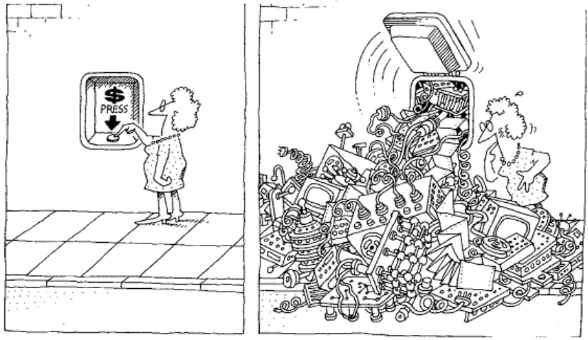
\includegraphics[width=0.5\textwidth]{complexityHiding.png}
\end{center}

Система сложна, существенная сложность может быть впечатляющей, но пользователю ничего знать про это не надо, ему система предоставляет возможно более простой интерфейс для решения его задач. Причём под пользователем тут понимается как конечный пользователь системы, так и коллеги-программисты, которые будут пользоваться написанным кодом, вызывать веб-сервисы и т.д.


\subsection{Модульность}

Лучший и наиболее широко используемый способ борьбы со сожностью программного обеспечения --- это разделение программы на модули. Принцип ``разделяй и властвуй'' применяется вообще повсюду, а модуль --- это способ разделить сложную задачу на менее сложные подзадачи, решить каждую подзадачу отдельно, а потом собрать из полученных решений решение исходной задачи.

Модульность как способ разбиения системы на компоненты, вообще говоря, позволяет создавать сколь угодно большие системы, поскольку модуль независим от других и общается с другими только через строго определённые интерфейсы. Разработку каждого модуля можно рассматривать как отдельную задачу, которая меньше по размеру, чем исходная. И проектировщик модуля уровнем выше может вообще ничего не знать про модули уровнем ниже кроме того, как их использовать --- что, если соблюдается принцип сокрытия сложности, не должно быть проблемой. Более того, разные модули могут разрабатываться разными людьми или командами, независимо друг от друга, пока все выполняют соглашения, прописанные в интерфейсах (как синтаксические, так и семантические --- неправильные типы аргументов поймает компилятор, а вот то, что, например, сначала надо вызвать Connect(), а потом уже GetData() --- вряд ли).

При разбиении на модули возникает вопрос, какого размера должен быть модуль, и даже принцип ``один модуль --- одна функциональность'' не всегда даёт ответ на этот вопрос. Начинающие программисты могут пихать вообще всё в один модуль, либо, столь же часто, делать кучу модулей по одной функции в каждом, думая, что вот, красивый модульный дизайн, минимизация интерфейсов и всё такое. Проблема в том, что если модули слишком большие, то сложность каждого модуля неоправданно велика, и, соответственно, неоправданно велики затраты на его разработку. Если модули слишком маленькие, то неоправданно велики затраты на их интеграцию --- модулей становится слишком много, взаимодействия между модулями становятся слишком сложны. В вырожденных случаях (один большой модуль или куча модулей по одной функции) мы никаких преимуществ от модульности вообще не получаем. Поэтому должен соблюдаться некоторый баланс:

\begin{center}
	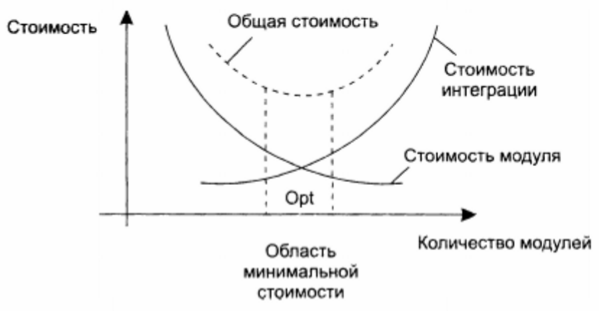
\includegraphics[width=0.5\textwidth]{modulesCost.png}
\end{center}

Есть знаменитое правило ``7+-2'', говорящее, что человек может одновременно удерживать в голове порядка семи сущностей (плюс-минус, в зависимости от индивидуальных способностей. Это правило может быть хорошей отправной точкой при проектировании системы и разбиении на модули.

Ещё хорошим показателем качества разбиени на модули могут быть численные метрики сопряжения и связности, которые можно просто посчитать (естественно, автоматически) для данного куска кода, или оценить на глаз. \textit{Сопряжение} (Coupling) --- мера того, насколько взаимосвязаны разные модули в программе (то есть насколько часто один модуль дёргает другие, насколько много этих других и насколько много они должны знать друг о друге). \textit{Связность} (Cohesion) --- мера того, насколько взаимосвязаны функции внутри модуля и насколько похожие задачи они решают. Целью при проектировании является слабое сопряжение (опять-таки, ``меньше знаешь --- крепче спишь'', можно независимо менять компоненты системы, не боясь всё сломать) и сильная связность (функции внутри модуля должны быть связаны друг с другом, иначе их следует разложить в отдельные модули --- прежде всего для того, чтобы модуль было проще понять и использовать).

Отдельно обращу внимание, что все эти хорошие практики направлены на упрощение понимания системы. И речь тут идёт не о понимании, которое может получить внимательный читатель, аккуратно разбираясь с каждой строчкой кода, а о понимании, которое необходимо, когда завтра релиз, а где-то в этих сотне тысяч строк кода есть критический баг, без исправления которого релиз не состоится, а код этот писала соседняя команда из Чехии, которая всем составом ушла в отпуск, и все комментарии на чешском.

\section{Объектно-ориентированное проектирование}

\subsection{Объекты}

В объектно-ориентированном проектировании роль модулей играют объекты и классы, а поскольку объектно-ориентированное программирование по сей день остаётся доминирующей парадигмой в промышленной разработке, дальше речь пойдёт про них. Впрочем, бывают объектно-ориентированные языки, не имеющие вовсе понятия ``класс'', так что поговорим сначала именно про объекты. Вот несколько разных определений из нескольких разных источников:

\begin{itemize}
	\item Objects may contain data, in the form of fields, often known as attributes; and code, in the form of procedures, often known as methods --- \textbf{\href{https://en.wikipedia.org/wiki/Object-oriented\_programming}{Wikipedia}}
	\item An object stores its state in fields and exposes its behavior through methods --- \textbf{\href{https://docs.oracle.com/javase/tutorial/java/concepts/object.html}{Oracle}}
	\item Each object looks quite a bit like a little computer --- it has a state, and it has operations that you can ask it to perform --- \textbf{\href{http://amzn.to/1PBmQpm}{Thinking in Java}}
	\item An object is some memory that holds a value of some type --- \textbf{\href{http://amzn.to/1XyGCtk}{The C++ Programming Language}}
	\item An object is the equivalent of the quanta from which the universe is constructed --- \textbf{\href{http://amzn.to/266oJr4}{Object Thinking}}
\end{itemize}

The C++ Programming Language подходит к определению объекта наиболее прагматично, потому что, вообще говоря, там это понятие нужно для описания семантики языка, а не для философских рассуждений, но вместе с тем такое определение самое бесполезное, поскольку перекладывает всю ответственность на понятие ``type''. Определения из Википедии и из доков по Java слишком механистичны и следуют традиции ошибочного понимания объектов как структур с методами --- технически это так, но не в этом суть понятия ``объект''. Больше всего соответствует этому курсу определение из Thinking in Java, объект как изолированная сущность, которая обладает каким-то поведением и может иметь состояние (что отличает объектно-ориентированное программирование от функционального). Object Thinking даёт слишком философское, хотя и совершенно в духе этого курса определение --- объект как единица декомпозиции объектно-ориентированной программы.

В любом случае, объекты имеют три важных свойства: состояние, поведение и идентичность. С состоянием связано такое важное понятие, как \textit{инвариант} --- набор логических условий, которые должны исполняться всё время жизни объекта. Инвариант важен, поскольку позволяет реализовывать методы будучи уверенными в том, что эти условия выполнены --- например, что количество элементов в связном списке равно значению поля length, что позволяет во всех методах, требующих просмотра всего списка, бежать просто от 0 до length и не думать, что будет, если следующий указатель null. Каждый объект сам отвечает за поддержание своего инварианта и обязан не давать возможности нарушить его извне (поэтому public-поля запрещены, например).

\subsection{Выделение абстракций}

Теперь надо обсудить, откуда, собственно, брать объекты и классы, если система ещё не написана. Допустим, у нас есть техническое задание, требующее разработать приложение для какой-то (возможно, незнакомой нам) предметной области. Тогда нашей первой задачей будет построение объектной модели предметной области и решаемой задачи, для чего обычно выполняются следующие действия:

\begin{enumerate}
	\item определение объектов и их атрибутов, чаще всего на основе общения с экспертами, самостоятельного изучения предметной области и здравого смысла --- часто встречающиеся существительные в речи экспертов, скорее всего, станут классами;
	\item определение действий, которые могут быть выполнены над каждым объектом (назначение ответственности) --- так же, слушаем экспертов и собираем информацию о предметной области, действия --- это глаголы;
	\item определение связей между объектами, задавая вопросы в духе ``а про это кто знает'', ``а это где используется'' и т.д.
	\item определение интерфейса каждого объекта, когда фиксируется и формализуется всё, что удаллось сделать на предыдущих этапах.
\end{enumerate}

Результатом этой деятельности будет первый грубый набросок архитектуры системы, выражаемый обычно в виде диаграммы классов:

\begin{center}
	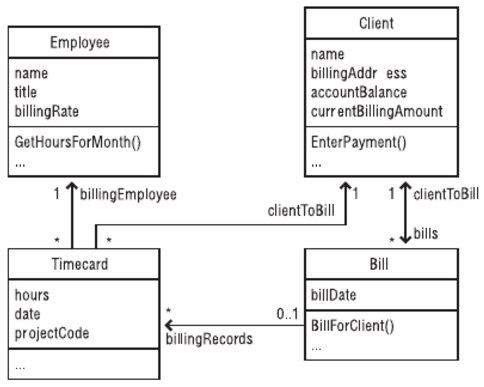
\includegraphics[width=0.55\textwidth]{billDomainModel.png}
\end{center}

Классы, конечно, появляются не только из предметной области, но и могут появляться в процессе реализации. Часто встречающиеся источники абстракций таковы:

\begin{itemize}
	\item изоляция сложности --- имеет смысл делать отдельными классами сложные алгоритмы, нетривиальные структуры данных, целые сложные подсистемы прятать за простыми фасадами. Делается это для того, чтобы, во-первых, спрятать сложность от остальной системы, во-вторых, иметь возможность менять алгоритмы, оптимизировать внутреннее представление и т.д., зная, что это ничего не сломает. При этом надо тщательно проектировать интерфейсы абстракций, скрыввающих сложность, потому что они имеют тенденцию сами становиться слишком сложными, что убивает все преимущества инкапсуляции.
	\item Изоляция возможных изменений --- прятать всё, что имеет большие шансы поменяться, в отдельный класс или подсистему, чтобы их можно было выкинуть и переписать, если изменение таки произойдёт. Однако не надо переусердствовать, хорошая архитектура позволяет себя менять и без специальной поддержки изменчивости. Основные источники изменений:
	\begin{itemize}
		\item бизнес-правила, то есть алгоритмы из предметной области, которые реализует программа, они меняются на удивление часто;
		\item зависимости от оборудования и операционной системы --- меняются редко, но изменение может быть критично для жизни программного продукта --- ваше любимое железо через пять лет, скорее всего, никто не будет выпускать, что при неаккуратном проектировании может потребовать переписать всю систему с нуля. Если вы думаете ``кому мой программный продукт будет нужен через пять лет'', вспомните (или почитайте) про проблему 2000 года;
		\item ввод-вывод, как формат файлов сохранения, так и формат сетевых пакетов, набор допустимых команд и т.д., они наверняка будут почему-то меняться;
		\item нестандартные возможности языка --- система должна иметь возможность пережить смену компилятора;
		\item сложные аспекты проектирования и конструирования --- это обсуждалось выше, сложность полезно прятать, но не только сложность реализации, но и сложность архитектуры --- сложные решения часто оказываются неверными, их должно быть можно легко поменять;
		\item третьесторонние компоненты --- нельзя критически зависеть от чего-то, что перестанет поддерживаться через полгода или станет стоить бешеных денег.
	\end{itemize}
	\item Изоляция служебной функциональности --- сущности, которые нужны для работы других сущностей. Это различного рода фабрики, репозитории, диспетчеры, медиаторы, сервисы (группы статических методов, полезных для работы) и т.д. и т.п. Классы, отвечающие за бизнес-логику, должны содержать только бизнес-логику, не захламляя её деталями реализации, детали должны жить отдельно.
\end{itemize}

\subsection{Принципы SOLID}

Есть пять базовых принципов объектно-ориентированного проектирования, известные как принципы SOLID. Эти принципы должны применяться при проектировании всех объектно-оориентированных систем, их любят спрашивать на собеседованиях, и вообще, их следовало бы рассказывать ещё на первом курсе, но обычно этого не делают.

Принципы таковы:

\begin{itemize}
	\item Single responsibility principle, принцип единственности ответственности --- каждый класс должен делать что-то одно. Кажется привлекательным иметь ``швейцарский нож'', который бы один решал все возможные проблемы, но такой класс, во-первых, тяжёл в сопровождении, а во-вторых, сложно понять его роль в системе, сложно объяснить её новым людям в проекте. Поэтому про каждый класс должно быть можно в одном предложении сказать, зачем он нужен, например, ``утилиты для работы со строками'', ``вычислялка процентов по вкладу''. И поэтому важно писать комментарии к самому классу --- ессли у вас не получается сформулировать кратко, что делает этот класс, значит, это плохая абстракция и её надо разбить на несколько классов. Ещё надо следить, чтобы ответственность класса была полностью инкапсулирована в этом классе. То есть, например, если у вас есть ``утилиты для работы со строками'' и ``ещё утилиты для работы со строками'', дела ваши плохи --- вы никогда в жизни не запомните где нужный вам метод. Это всё касается не только классов, но и функций, и целых подсистем.
	\item Open/closed principle, принцип открытости/закрытости --- абстракция (класс, модуль, функция) должна быть открыта для расширения, но закрыта для изменения. То есть, если интерфейс уже стабилизировался и им начали пользоваться, менять его нельзя. Если надо добавить в абстракцию новую функциональность, можно использовать наследование и/или заранее подготовленные точки расширения, как на картинке:
		\begin{center}
			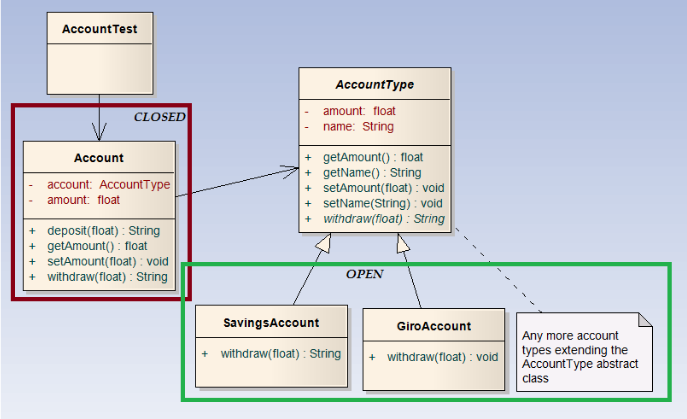
\includegraphics[width=0.5\textwidth]{openClosedPrinciple.png}
		\end{center}

		Если это правило не соблюдать, интерфейс абстракции начнёт увеличиваться в размерах, сам собой начнёт нарушаться принцип единственности ответственности, и в результате мы получим несопровождаемого и неюзабельного монстра (см. антипаттерны ``God object'' и ``Swiss army knife'' далее в этом курсе).
	\item Liskov substitution principle, принцип подстановки Барбары Лисков --- то самое определение наследования, о котором шла речь выше. Функции, которые используют базовый тип, должны иметь возможность использовать подтипы базового типа, не зная об этом. Это означает, в частности, что классы-потомки должны реализовывать интерфейсы классов предков (как чисто синтаксически, так и семантически --- делать то, что ожидается от предка) и, про что часто забывают, выполнять все инварианты классов-предков, явные или неявные. Хороший пример проблем с принципом подстановки --- проверяемые исключения в Java. Методы класса-предка могли задекларировать исключения, которые они могут бросать, тогда потомок, переопределяющий эти методы, имел право бросать только эти исключения. Почему --- вызывающий мог использовать try/catch для обработки ошибок, и если там были написаны catch-блоки для исключений предка, а потомок бросал что-то новое, это ломало вызывающего и тем самым нарушало принцип подстановки. Компилятор проверял такие ситуации и сообщал об ошибке, если потомок пытался бросить незадекларированное в предке проверяемое исключение. Проблема в том, что в большинстве случаев заранее предсказать все исключительные ситуации, которые могут возникнуть в потомках, при написании предка невозможно, поэтому проверяемые исключения особо не используются нынче в Java и так и не попали ни в один другой язык.
		\begin{center}
			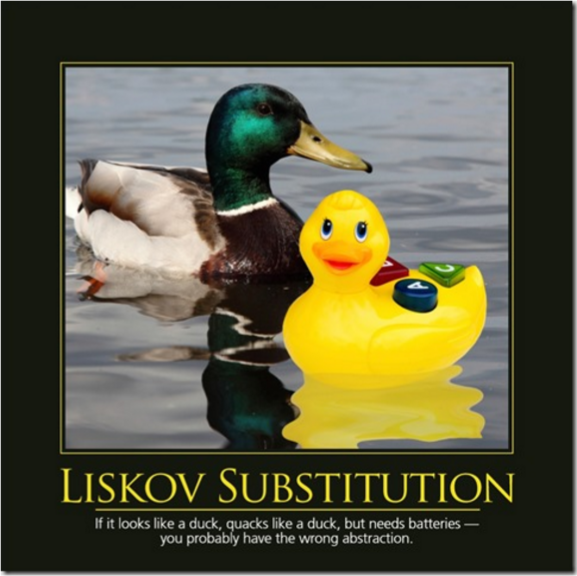
\includegraphics[width=0.4\textwidth]{liskovSubstitutionPrinciple.png}
		\end{center}
	\item Interface segregation principle, принцип разделения интерфейсов --- клиенты не должны зависеть от методов, которые они не используют. Если у абстракции есть группы методов, нужные разным клиентам, то имеет смысл сделать разные интерфейсы, по одному на каждую группу методов. Например, у нас есть модем (например, 4G/LTE), который умеет устанавливать соединение и при наличии соединения передавать данные. У нас есть системная утилита установки соединения, которая следит за сотовой сетью и устанавливает соединение, если это возможно, и у нас есть сетевой стек, который передаёт данные, если его попросят. Если просто сделать интерфейс IModem, который будет името методы Connect() и Send(), это как раз нарушит принцип разделения интерфейсов, потому что утилиту установки соединения надо будет пересобирать каждый раз, когда меняются параметры метода Send(), который ей совсем не нужен, а сетевой стек придётся пересобирать каждый раз, когда меняется Connect(), который в этом примере сетевой стек не использует (например, потому, что не хочет знать подробности сотовой связи). Необходимость разделять интерфейсы абстракции, впрочем, может указывать на нарушение принципа единственности ответственности, но может и нет (в нашем примере ``модем'' был единой сущностью и в этом плане всё было ок, просто клиенты использовали его по-разному). Ещё важно не переусердствовать, ведь формально у класса должно быть ровно столько интерфейсов, сколько клиентов его используют, но это бессмысленно и опасно в плане излишних зависимостей. Группировать в интерфейсы надо методы, которые реально кластеризуются по смыслу, а не чисто механически.
		\begin{center}
			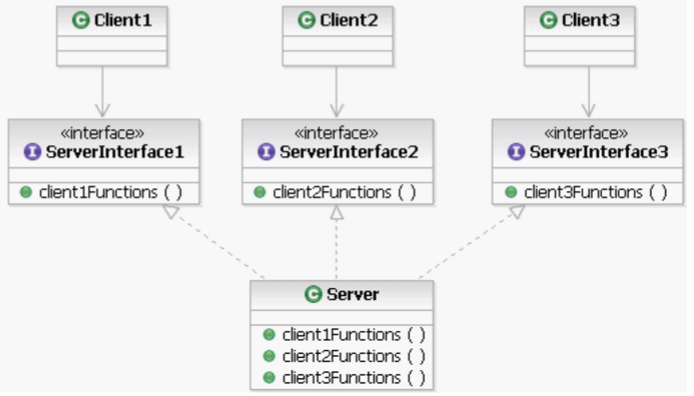
\includegraphics[width=0.5\textwidth]{interfaceSegregationPrinciple.png}
		\end{center}
	\item Dependency inversion principle, принцип инверсии зависимостей --- модули верхних уровней не должны зависеть от модулей нижних уровней, оба типа модулей должны зависеть от абстракций. Эту фразу, бывает, студенты выучивают наизусть и повторяют на экзамене как заклинание, совершенно не понимая её смысла. Проще всего пояснить суть дела на примере:
		\begin{center}
			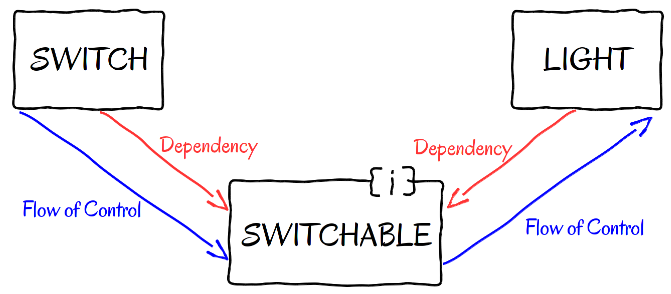
\includegraphics[width=0.5\textwidth]{dependencyInversionPrinciple.png}
		\end{center}

		Положим, у нас есть выключатель, который управляет лампочкой. Наивным решением было бы сделать класс Switch, у которого было бы поле типа Light (лампочка), и он бы вызывал её методы on()/off(). Чем это плохо --- выключатель может управлять только лампочкой, выключатель надо перекомпилировать, когда меняется лампочка, работу выключателя невозможно понять, не зная про лампочку. Если выключатель ещё и сам создаёт лампочку, невозможно подсунуть вместо неё mock-объект, что затрудняет тестирование. Правильное решение (та самая инверсия зависимостей) --- сделать интерфейс ``то, что можно включать/выключать'' (Switchable), сделать так, чтобы лампочка реализовывала этот интерфейс и сделать в классе Switch поле типа Switchable, так, чтобы он вообще ничего про лампочку не знал. Тпереь выключатель сам объект-лампочку создать в принципе не может (он просто не знает, что она есть), так что должен получать свою зависимость либо параметром в конструктор, либо в метод-сеттер (что называется Dependency Injection, внедрение зависимости). Кстати, существуют и активно используются целые библиотеки, занимающиеся управлением зависимостями и инициализацией объектов, так называемые IoC-контейнеры (Inversion of Control), без них не обходится ни одна современная библиотека для разработки веб-приложений, например. Тем не менее, и без библиотек это хорошая практика, существенно уменьшающая зависимости между модулями программы.
\end{itemize}

\subsection{Закон Деметры}

Ещё одно хорошее правило, не являющееся частью принципов SOLID --- это закон Деметры, кратко формулирующийся как ``Не разговаривай с незнакомцами''. Более формально, правило говорит о том, что объект A не должен иметь возможность получить непосредственный доступ к объекту C, если у объекта A есть доступ к объекту B, и у объекта B есть доступ к объекту C. Например,

\begin{minted}{java}
book.pages.last.text  // Плохо
book.pages().last().text()  // Лучше, но тоже не супер
book.lastPageText()  // Идеально
\end{minted}

Почему так --- вызовы ``по цепочке'' раскрывают внутреннюю структуру данных класса и не дают её потом изменить. В нашем примере с книгой цепочка вызовов говорит, что в книге есть коллекция страниц, у которой обязательно есть метод last() (и любая другая коллекция без этого метода не подойдёт), и что там лежат страницы, у которых есть метод text(). Если мы хотим просто полуить текст последней страницы, это ну очень много знаний, которые нам не нужны и заставляют нас зависеть от автора класса-книги. В книжке Р. Мартина ``Чистый код'' проводится аналогия с крушением поезда --- где-то посреди структуры меняется внутреннее представление и всё, все эти цепочки вызовов надо переделывать.

Как обычно, главное не переусердствовать. Код вида book.firstPageText(), book.secondPageText(), book.thirddPageText() и т.д. гораздо хуже, чем ``паровозик''. Закон Деметры говорит просто, что не надо выставлять напоказ структуру данных, которая не является частью абстракции, и если мы реально ожидаем доступ к каждой странице (что, вообще говоря, для книги вполне ок), то имеет смысл предоставить-таки коллекцию pages(). Более того, с нарушением закона Деметры часто путают очень полезный приём программирования ``Fluent API'', когда через точку пишется последовательность действий, которые надо выполнить над объектом (хороший пример --- это Java Stream API или LINQ в .NET), этот же приём используется в паттерне ``Строитель'', про который тоже будет в этом курсе. Здесь с законом Деметры всё ок, потому что цепочка fluent-вызовов, как правило, возвращает один и тот же объект, не раскрывая его внутренней структуры (любители функционального программирования могут провести параллели с монадами, и на самом деле LINQ проектировался как самые настоящие монады на C\#).

\section{Некоторые принципы хорошего кода}

Теперь перейдём от абстрактных рассуждений к конкретным примерам кода и соображениям по поводу ``тактического'' проектирования, помогающим писать расширяемый и сопровождаемый код. Далее будет на самом деле краткий обзор книжек Р. Мартина ``Чистый код'' и ``Code Complete'' С. Макконелла, которые, впрочем, рекомендуются к прочтению --- они не очень большие, легко читаются и могут научить куче полезных приёмов.

\subsection{Абстракция}

Начнём мы с абстракции, как самого важного из ``китов'' ООП, хоть её редко упоминают в таковом качестве.

Рассмотрим пример. У нас есть объект ``Шрифт'' и мы хотим уметь менять ему размер. Вот так это можно было бы сделать:

\begin{itemize}
	\item \mintinline{java}|currentFont.size = 16| --- прямое присвоение полю, ужасно. Во-первых, шрифт не может поддерживать свой инвариант и изменить внутреннее представление размера. Во-вторых, тут написано ``размеру присвоить 16''. Окей, чего 16? Ну а чего размеру?
	\item \mintinline{java}|currentFont.size = PointsToPixels(12)| --- чуть лучше. Теперь размер, видимо, измеряется в пикселях.
	\item \mintinline{java}|currentFont.sizeInPixels = PointsToPixels(12)| --- ещё чуть лучше. Теперь про размер явно написано, что он измеряется в пикселях.
	\item \mintinline{java}|currentFont.setSizeInPoints(sizeInPoints)| \newline
			\mintinline{java}|currentFont.setSizeInPixels(sizeInPixels)| --- совсем хорошо. Нам-то какое дело, в чём внутри у шрифта измеряется размер, мы хотим его выставлять в тех единицах измерения, которые нам удобны.
\end{itemize}

Ещё один небольшой пример, обычного класса на Java, который умеет, видимо, что-то исполнять и печатать по этому делу отчёты:

\begin{minted}{java}
public class Program {
    public void initializeCommandStack() { ... }
    public void pushCommand(Command command) { ... }
    public Command popCommand() { ... }
    public void shutdownCommandStack() { ... }
    public void initializeReportFormatting() { ... }
    public void formatReport(Report report) { ... }
    public void printReport(Report report) { ... }
    public void initializeGlobalData() { ... }
    public void shutdownGlobalData() { ... }
}
\end{minted}

Тут никаких полей нет, имена методов и параметров адекватны, но всё равно этот класс ужасен. Потому что нарушает принцип единственности ответственности. Он умеет и что-то делать со стеком команд, и с отчётами, и с глобальными данными, так что непонятно, когда и как им пользоваться. Про этот класс нельзя одним предложением сказать, что он такое. Чтобы сделать этот класс хорошим, его неплохо бы распилить на три --- стек команд, управлялка отчётами и хранилище глобальных данных. И добавить четвёртый класс, который бы управлял этими тремя классами. И это не будет овердизайном, потому что тут и так на самом деле три класса, просто они упиханы в один.

Вот другой класс на Java, представляющий сотрудника какой-то компании:

\begin{minted}{java}
public class Employee {
    public Employee(
            FullName name,
            String address,
            String workPhone,
            String homePhone,
            TaxId taxIdNumber,
            JobClassification jobClass
    ) { ... }

    public FullName getName() { ... }
    public String getAddress() { ... }
    public String getWorkPhone() { ... }
    public String getHomePhone() { ... }
    public TaxId getTaxIdNumber() { ... }
    public JobClassification getJobClassification() { ... }
}
\end{minted}

У этого класса с абстракцией всё хорошо, он занимается ровно одним делом (представляет сотрудника компании), все имена понятны. Кроме того, тут используется ещё один хороший для абстракции приём --- специальные типы для значений. Например, TaxId вполне может быть классом с ровно одним полем типа String, геттером и сеттером, и всё. Зато теперь тут скрыто внутреннее представление TaxId (и его легко можно переделать на int, если окажется, что это возможно) и компилятор поругается, если мы перепутаем порядок аргументов. FullName может быть несколько более сложной штукой, там может быть фамилия, имя и отчество. Мы это всё тоже могли бы передавать в конструктор Employee как три отдельные строки, но зачем, ведь FullName --- это концептуально целостная штука. Достоинства такого подхода понятны, недостатки тоже --- за абстракцию и большую надёжность мы платим строками кода. Стоит ли платить эту цену --- приходится решать в каждом конкретном случае. Отметим, что в функциональных языках объявить тип обычно гораздо менее трудозатратно, чем в Java, так что там таким приёмом пользуются часто и с удовольствием.

В продолжение темы платы строками кода за качество абстракции ещё один пример:

\begin{minted}{java}
public class Point {
    public double x;
    public double y;
}
\end{minted}

против

\begin{minted}{java}
public interface Point {
    double getX();
    double getY();
    void setCartesian(double x, double y);
    double getR();
    double getTheta();
    void setPolar(double r, double theta);
}
\end{minted}

Тут мы видим, что поскольку в Java нет структур, то приходится объявлять классы, и чтобы не писать ненужных геттеров/сеттеров, можно сразу объявить public-поля, потому что по смыслу это структура, инвариантов у неё нет, и использовать её предполагается только как хранилище данных. Тем не менее, несмотря на большую многословность, второй вариант более архитектурно правильный, потому что обладает интересным свойством --- тут вообще нигде не написано, как точка представляется внутри. Мы можем трактовать точку как точку в декартовых координатах, можем --- как в полярных, ей всё равно. Для этого, кстати, геттеры позволяют получить каждую координату отдельно, но сеттеры позволяют выставить только обе координаты сразу --- позволять менять координаты по одной было бы странно с точки зрения семантики операций с учётом того, что изначально точка могла задаваться в другой системе координат. Кстати, этот пример показателен не только для Java, где всё очень плохо, но и для C\#, где есть и структуры и свойства --- первая абстракция всё равно отличается от второй тем, что она ``недостаточно абстрактна''. Нужна ли нам большая абстрактность или это приведёт к овердизайну --- вопрос, на который должен ответить архитектор, опять-таки, для каждого конкретного случая.

Следующее соображение, влияющее на качество абстракции --- это её ``уровень'' и консистентность этого уровня по абстракции. Например:

\begin{minted}{java}
public class EmployeeRoster implements MyList<Employee> {
    public void addEmployee(Employee employee) { ... }
    public void removeEmployee(Employee employee) { ... }
    public Employee nextItemInList() { ... }
    public Employee firstItem() { ... }
    public Employee lastItem() { ... }
}
\end{minted}

Тут принцип единственности ответственности соблюдается --- это список сотрудников какой-то компании, всё хорошо. Наследование используется по делу, список сотрудников определённо является списком. Имена и параметры тоже адекватны --- можно добавить сотрудника, получить сотрудника, удалить сотрудника, вроде всё ок. Тем не менее, сравним это со вторым классом:

\begin{minted}{java}
public class EmployeeRoster {
    public void addEmployee(Employee employee) { ... }
    public void removeEmployee(Employee employee) { ... }
    public Employee nextEmployee() { ... }
    public Employee firstEmployee() { ... }
    public Employee lastEmployee() { ... }
}
\end{minted}

Тут мы уже не наследуемся от списка (о ужас, теперь для нашего класса не будут работать библиотечные алгоритмы, работающие над списками) и переименовали пару методов. Стало лучше? Гм, рассмотрим ещё один пример --- в стандартной библиотеке Java долгое время стек наследовался от списка. Ну а что, стек --- это список с методами push и pop. Теперь это каноничный пример плохого дизайна --- стек, конечно, не список, потому что не должен получать от списка пачку методов, ломающих инварианты стека. Но суть даже не в инвариантах, а в том, что стек --- это что-то простое, список --- это что-то сложное и предназначенное не для того. Возвращаясь к нашему примеру, список сотрудников --- это что-то сложное и техническое, у него есть методы для итерирования (nextItemInList, firstItem и lastItem) и мало ли что ещё. А мы хотим просто список сотрудников, мы не хотим итератор или какой-нибудь сплитератор, если речь идёт о Java (может, мы двенадцатилетний сын директора компании, который пишет на Питоне автоматизацию начисления зарплаты). Поэтому хорошая абстракция часто вынуждена не расширять уже существующую, а прятать её и предоставлять более простой интерфейс, даже несмотря на то, что это усложнит переиспользование кода. Задача абстракции --- быть удобной для использования и для понимания, а не уметь делать много всего. При этом удобство понимания важнее.

Есть некоторый набор общих рекомендаций, про которые тоже неплохо бы помнить, проектируя свои классы и интерфейсы.

\begin{itemize}
	\item Про каждый класс знайте, реализацией какой абстракции он является. Принцип единственности ответственности имеет очень простой критерий --- если про класс можно одним коротким предложением сказать, что он такое, то всё ок. Может потребоваться разделить класс на несколько разных классов просто потому, что методы по смыслу слабо связаны, и это будет не овердизайн, как мы видели ещё в первом примере.
	\item Учитывайте противоположные методы (add/remove, on/off, ...). Даже если они сейчас не нужны, когда-то кому-то неизбежно понадобятся.
	\item Разделяйте команды и запросы, избегайте побочных эффектов. Команда только меняет состояние, не возвращая результат, запрос только возвращает результат, не меняяя состояния. Это хорошо как для понимания программы, так и по более прагматичному соображению --- в многопоточной программе синхронизации требуют только команды. Сколько угодно запросов может исполняться параллельно.
	\item Не возвращайте null. null всегда сюрприз для вызывающего, даже если он прекрасно знает, что любой ссылочный тип может иметь значение null. Возвращайте Option --- это вынудит вызывающего явно проверить наличие значения. Ну или бросайте исключение, если null-ы бывают только если что-то пошло не так.
	\item По возможности делайте некорректные состояния невыразимыми в системе типов. Это особо хорошо работает в функциональных языках, потому что там мощные системы типов, но и в других языках систему типов можно заставить работать на себя --- вспомните второй пример, с TaxId и FullName у Employee.
	\item Семантику языка тоже надо заставить работать на себя в плане чистоты абстракций. Самый простой пример --- комментарии в духе ``не пользуйтесь объектом, не вызвав  init()'' можно заменить конструктором. Вообще, всё, что не проверяется компилятором, будет использовано неправильно, так что надо стараться так, чтобы вашей абстракцией пользоваться неправильно было просто невозможно.
	\item При рефакторинге надо следить, чтобы интерфейсы не деградировали. Рефакторинг --- опасная вещь, потому что в погоне за тактической выгодой типа скорости работы или удобства вызовов можно потерять стратегические преимущества хороших абстракций.
\end{itemize}

\subsection{Инкапсуляция}

Следующее важное понятие в ООП --- это инкапсуляция. Под которым обычно понимают сокрытие деталей реализации, несмотря на то, что инкапсуляция --- это обычно просто свойство кода, относящегося к одной задаче, лежать рядом. В принципе, в ООП и инкапсуляция в этом понимании, и сокрытие деталей реализации обеспечиваются классами (либо чем-то похожим), так что всё вместе называть инкапсуляцией вполне валидно.

Инкапсуляция --- это механизм защиты инвариантов объекта на самом деле. Из этого следует, во-первых, принцип минимизации доступности методов, который коротко формулируется как ``меньше знаешь --- крепче спишь''. Чем меньше интерфейс объекта, тем проще им пользоваться и тем проще уследить за инвариантами объекта. С другой стороны, тем меньше объект умеет делать, но это даже хорошо --- принцип единственности ответственности и всё такое. Другое дело, что если у всех объектов ровно по одному методу (как в функциональных программах, например), то это не идеальная инкапсуляция, а наоборот печаль, потому что сложность переносится из объектов во взаимодействие между объектами.

Во-вторых, из этого следует, что паблик-полей не бывает. Паблик-поля вообще не могут поддерживать никаких инвариантов, поэтому, скорее всего, просто не относятся к тому классу, в котором объявлены. Это, конечно, вызывает вопросы ``А что делать, если класс не имеет инвариантов и так, например, используется только для передачи данных?''. Например,

\begin{minted}{java}
class Point {
    public float x;
    public float y;
    public float z;
}
\end{minted}

и

\begin{minted}{java}
class Point {
    private float x;
    private float y;
    private float z;
    public float getX() { ... }
    public float getY() { ... }
    public float getZ() { ... }
    public void setX(float x) { ... }
    public void setY(float y) { ... }
    public void setZ(float z) { ... }
}
\end{minted}

По этому поводу бывают разные мнения, во многих языках есть структуры специально для таких дел, но в целом сообщество сходится на том, что второй вариант предпочтительнее, несмотря на то, что его стоимость в строках кода в разы выше. Почему --- код, к несчастью, имеет свойство развиваться, так что то, что раньше было просто классом для передачи данных без инвариантов или чего бы то ни было, внезапно становится полноценной абстракцией с кучей методов, инвариантов и т.д. и т.п. Геттеры с сеттерами легко подправить так, чтобы они начали делать что-то умное, поля --- придётся переписывать весь код, использующий наш класс.

Ещё некоторые рекомендации касательно инкапсуляции.

\begin{itemize}
	\item Класс не должен ничего знать о своих клиентах. Образ мыслей ``а здесь я не буду вставлять проверку на null, потому что из моего кода его никто с null не вызывает'' неправильный, это нарушение инкапсуляции ``с другой стороны'' (когда не внешний мир лезет в класс, а класс чего-то хочет от внешнего мира). Всё сломается, когда ваш класс захотят переиспользовать где-то ещё.
	\item Лёгкость чтения кода важнее, чем удобство его написания. Написать код надо один раз (при этом IDE будет помогать всякими автодополнениями), а читать его придётся, быть может, тысячи раз разным людям.
	\item Опасайтесь семантических нарушений инкапсуляции, например, ``не будем вызывать ConnectToDB(), потому что GetRow() сам его вызовет, если соединение не установлено''. Даже если это правда, это предположение о том, как реализована абстракция, или программирование \textit{сквозь} интерфейс.
	\item Protected- и package- полей тоже не бывает. На самом деле, у класса два интерфейса --- для внешних объектов и для потомков (может быть отдельно третий, для классов внутри пакета, но это может быть плохо). Все эти интерфейсы должны быть полноценными интерфейсами, то есть защищать инварианты, поддерживать контракты и т.д. Потомков вы вообще не контролируете и доверять им нельзя, классы внутри пакета безопаснее, но тоже никто не сказал, что ваш пакет будете всегда разрабатывать только вы и только в непомутнённом состоянии рассудка.
\end{itemize}

\subsection{Наследование и полиморфизм}

Наследование хоть и считается одним из трёх китов, на которых зиждется ООП, современная архитектурная мысль считает его очень нишевым и довольно неуклюжим инструментом. Наследование почти всегда может быть заменено на агрегацию с делегированием запросов агрегируемому объекту, и на самом деле внутри в большинстве языков программирования наследование реализуется именно так --- класс-потомок просто имеет внутри себя объект класса-предка, методы которого можно вызывать по интерфейсу потомка. Агрегация или композиция имеют ряд преимуществ над наследованием, основное из которых --- возможность переконфигурирования во время выполнения. Наследование фиксируется во время компиляции и требуется перекомпилировать программу, чтобы поменять предка, в поле можно просто положить новый объект прямо в процессе работы. Даже во время компиляции наследование не очень гибко --- в разных языках есть ограничения на количество классов-предков, всякое ромбовидное наследование и тонкости, с ним связанные, и т.д. Агрегация лишена этих недостатков. У агрегации тоже есть проблемы --- во-первых, это чисто синтаксически необходимость явно описывать в нашем классе все методы, которые мы хотим поддержать, и реализовывать их перенаправлением запроса агрегируемому объекту (опять-таки, больше строк кода). Во-вторых, с агрегацией не работает полиморфизм (хотя если сам агрегируемый объект полиморфный, можно добиться ряда занятных эффектов, см. паттерны ``Состояние'' и ``Стратегия'').

Поэтому в целом можно сказать, что наследование имеет смысл использовать только для обеспечения полиморфизма. Наследование для переиспользования общей функциональности предка можно смело заменять на включение этого ``предка'' как поля во все классы, которым нужна его функциональность. А это, в свою очередь, значит, что наследоваться от конкретных (и даже абстрактных) классов нет никакой нужды --- интерфейсов для обеспечения полиморфизма вполне достаточно, а переиспользовать код предка всё равно плохо. Из этого, в свою очередь, следует, что private-наследование, как оно реализовано в C++, суть ересь. И C++ настолько ужасен, что наследование в нём private по умолчанию. Впрочем, по моему опыту, private-наследование в реальном промышленном коде на C++ используется крайне редко.

На самом деле, заявления выше несколько категоричны. Есть способы использования наследования для обеспечения конфигурирования класса-предка --- см., например, паттерн ``Шаблонный метод'' или большинство оконных библиотек. Там основная функциональность реализуется в классе-предке, потомки нужны, чтобы переопределить виртуальные методы предка так, чтобы всё вместе делало что-то полезное. Впрочем, большинство таких вещей писалось до массового распространения лямбда-функций в языках программирования, так что по-другому делать было просто очень неудобно. Возможно, мы скоро увидим фреймворки, которые наследованием не пользуются вовсе.

Наследование --- по определению отношение ``является'' между типами. Есть простой способ проверки иерархии наследования на адекватность --- принцип подстановки Барбары Лисков: любой код, который может работать с предком, должен мочь работать и с потомком. То есть наследование --- это наследование интерфейса (в смысле обеспечения полиморфизма подтипов), причём интерфейса в широком смысле --- обязательств и инвариантов.

Многие языки позволяют явно запретить наследование (final- или sealed-классы, final-методы). Есть две школы мысли по поводу того, как это использовать. Некоторые библиотекописатели (например, Microsoft) считают, что в библиотечном коде запрещать наследование нельзя, потому что это существенно ограничивает гибкость. Где-то в документации от Microsoft приводился пример с подключением к базе данных, где наследование от библиотечного класса использовалось только для того, чтобы определить конструктор, подставляющий нужный Connection String, и это типа удобно. Некоторые наоборот считают, что всё, для чего наследование не разрешено явно, должно быть закрыто для наследования, потому что если вы хотите позволить наследоваться от вашего класса, вам надо подумать о защите ваших инвариантов от потомков, о правильном использовании потомками методов вашего класса и т.д., это некоторая работа и делать её для каждого класса смысла нет.

Некоторые code smells, которые намекают на то, что с иерархией наследования что-то не так:

\begin{itemize}
	\item базовый класс, у которого только один потомок; оставлять возможности для расширения ``на будущее'', которое никогда не наступит, не стоит, благо в будущем можно и отнаследоваться, если будет надо, это не страшный рефакторинг;
	\item пустые переопределения --- предок декларирует контракты, которые потомок не может содержательно выполнить;
	\item очень много уровней в иерархии наследования --- обычно больше семи уровней означает, что всё совсем плохо, три-четыре уровня --- подозрительно; бывают исключения, например, иерархия наследования в абстрактном синтаксическом дереве компилятора;
	\item новые методы с такими же именами, как у родителей --- во-первых, это путает пользователя, во-вторых, это сильный индикатор того, что потомок вовсе потомком не является, а делает что-то своё.
\end{itemize}

Бывает, что наследование не используется там, где использоваться должно бы. Самый явный индикатор этого --- switch или длинная цепочка из if-else, где в зависимости от значения какого-то поля выбирается какое-то действие. Это на самом деле попытка реализовать вручную таблицу виртуальных методов. Простой пример:

\begin{minted}{java}
class Operation {
    private char sign = '+';
    private int left;
    private int right;

    public int eval() {
        switch (sign) {
            case '+': return left + right;
            case '-': return left - right;
        }
        throw new RuntimeException();
    }
}
\end{minted}

Это легко можно заменить на виртуальный вызов, где роль того поля, по которому делается выбор, играет тип времени выполнения объекта, у которого этот виртуальный вызов делается:

\begin{minted}{java}
abstract class Operation {
    private int left;
    private int right;

    protected int getLeft() { return left; }
    protected int getRight() { return right; }
    abstract public int eval();
}

class Plus extends Operation {
    @Override public int eval() { 
        return getLeft() + getRight(); 
    }
}

class Minus extends Operation {
    @Override public int eval() { 
        return getLeft() - getRight(); 
    }
}
\end{minted}

Опять-таки, кода становится больше, но архитектура в целом становится лучше --- теперь нет switch-а, который вынужден знать про все возможные операции, набор операций несложно расширить, теперь они могут быть довольно сложными (вплоть до того, чтоы собираться из элементарных операций в рантайме, см. паттерн ``Интерпретатор''). И операции в процессе развития программы могут получить ещё какую-нибудь ответственность, например, ``печатать себя'', и это будет очень легко поддержать, не городя ещё один гигантский switch.

\subsection{Вопросы инициализации}

Особого внимания заслуживают вопросы создания и инициализации объектов (и, что более интересно, сложных конструкций из нескольких объектов). Касательно конструкторов рекомендации такие:

\begin{itemize}
	\item Инициализируйте все поля, которые надо инициализировать. Конструктор --- это тот код, который более-менее обязательно выполняется при создании объекта, поэтому его задача --- сделать так, чтобы все инварианты после него выполнялись. Надеяться на то, что пользователь честно-честно вызовет метод init() после конструктора --- бессмысленно.
	\item Не вызывайте виртуальные методы из конструктора. Обычно вам даже компилятор скажет, что вы неправы, но если нет, последствия могут быть печальны. Дело в том, что при создании объекта конструкторы вызываются по цепочке, соответствующей иерархии наследования, при этом сначала вызываются конструкторы предка. Так что если ваш любимый язык таки позволяет сделать виртуальный вызов, вызовется метод потомка ещё до того, как конструктор потомка будет иметь шанс установить свои инварианты.
	\item Используйте private-конструкторы для объектов, которые не должны быть созданы, или одиночек (некоторые языки позволяют явно сказать, что конструктора нет --- \mintinline{cpp}|= delete;| в C++, abstract в C\# и Java), используйте protected-конструкторы для абстрактных классов --- создать их всё равно нельзя, так что нечего смущать пользователя, но из потомков вызывать конструктор может быть нужно.
	\item Одиночек надо использовать с большой осторожностью, потому как это замаскированные глобальные переменные со всеми вытекающими проблемами.
	\item Deep copy предпочтительнее Shallow copy, хотя второе может быть эффективнее. Пользователи в любом случае ожидают семантику глубокого копирования и могут быть удивлены, если изменения одного объекта приведут к изменению и другого. Глубокое копирование может быть сложным в реализации, если речь идёт про большой граф объектов, особенно если надо разбираться с идентичностью объектов (если объекты хранятся в БД или передаются по сети, их идентичность определяется не их местом в памяти, так что о ней надо думать при копировании). Если с идентичностью проблем нет, можно использовать такой хак --- сериализовать копируемый объект в поток байт в памяти, потом десериализовать.
\end{itemize}

\subsection{О мутабельности}

Мутабельность --- способность объекта изменять своё состояние --- довольно важное свойство, оказывающее существенное влияние на архитектуру. Если кратко, то мутабельное состояние --- это плохо и его надо стараться избегать. Более подробно, мутабельность запутывает причинно-следственные связи в программе --- кто-то вызвал метод, меняющий состояние, потом кто-то ещё, потом объект ведёт себя не так, как ожидалось. Кроме того, мутабельность создаёт дополнительные сложности для многопоточного программирования --- если состояние можно изменять, надо следить, чтобы два потока не пытались его изменить одновременно.

Тем не менее, основные современные языки программирования предполагают, что состояние мутабельно по умолчанию, а иногда (например, в Java) надо ещё помучаться, чтобы сделать класс немутабельным. Вот про что надо помнить, делая немутабельный класс.

\begin{itemize}
	\item Не предоставлять методы, модифицирующие состояние. Часто модификация состояния по смыслу всё-таки нужна, но есть полезный приём --- заменить модифицирующие состояние методы на методы, возвращающие копию объекта. При этом, разумеется, поменяется семантика программы, так что это не чисто механическое изменение.
	\item Не разрешать наследоваться от класса.
	\item Сделать все поля константными.
	\item Не давать никому ссылок на поля мутабельных типов. Даже если поля константны, константное поле мутабельного ссылочного типа не позволяет только модифицировать саму ссылку, объект, на который она указывает --- сколько угодно.
\end{itemize}

Правила хорошего тона говорят, что немутабельным должно быть всё, что может быть немутабельным без существенного вреда смыслу или скорости работы программы.

\subsection{Об оптимизации}

Кстати, по поводу скорости работы программы:

\textit{Во имя эффективности (без обязательности ее достижения) делается больше вычислительных ошибок, чем по каким-либо иным причинам, включая непроходимую тупость.} \newline
-- William A. Wulf 

\textit{Мы обязаны забывать о мелких усовершенствованиях, ска­жем, на 97\% рабочего времени: опрометчивая оптимизация --- корень всех зол.} \newline
-- Donald E. Knuth

\textit{Что касается оптимизации, то мы следуем двум правилам: \newline
Правило 1. Не делайте этого. \newline
Правило 2 (только для экспертов). Пока не делайте этого -- т.е. пока у вас нет абсолютно четкого, но неоптимизированного решения.} \newline
-- M. A. Jackson

В общем, скорость работы программы не так важна, как её объясняющая способность. Часто она вообще не имеет значения --- время реакции пользователя составляет сотни миллисекунд, так что 20 миллисекунд вы сортируете массив или 40, вообще не важно, если это надо сделать один раз по клику на кнопку. Для любителей спортивного программирования стремление по умолчанию писать ``оптимальный'' код может послужить причиной больших проблем с сопровождаемостью при довольно незначительном выигрыше в скорости работы. В общем, во-первых, надо себя сдерживать и стараться предпочитать простое решение быстро работающему (ну, до разумных пределов, всё-таки выбирайте алгоритм с подходящей асимптотикой, не надо числа Фибоначчи рекурсивно считать). Во-вторых, тонкой настройкой производительности (типа управления сборкой мусора и т.п.) надо заниматься \textit{только} после исследования системы профилятором. Впрочем, есть противоположное оптимизации понятие --- ``пессимизация'', означащее откровенную глупость, приводящую к замедлению программы (типа случайного boxing-а внутри цикла в Java), этого тоже надо избегать.

\subsection{Общие рекомендации}

Наконец, общие рекомендации по поводу написания качественного кода, которые в другие разделы не попали:

\begin{itemize}
	\item Fail Fast. Казалось бы, если программа падает, то это плохо. На самом деле, гораздо лучше, если программа упадёт, чем если продолжит работу в некорректном состоянии и испортит пользовательские данные. Поэтому принцип ``Fail Fast'' говорит, что программа должна завершить работу при малейшем подозрении на ошибку, а программист должен прикладывать усилия при написании кода, чтобы обнаружить потенциальную ошибку как можно раньше. Например, сильно помогает активное использование assert-ов. Чем их больше, тем лучше --- можно проверять инварианты, предусловия и постусловия методов, любые предположения и всё-всё-всё. Если есть языковые или библиотечные средства, позволяющие явно декларировать контракты или nullability, ими надо пользоваться (даже если это лишний код, замедляет рефакторинг и всё такое). Ещё полезный приём --- ``Защитное программирование'', когда ваш код не доверяет адекватности всего, что вовне --- например, проверяет каждый параметр каждого public-метода на корректность. Не надо выключать проверки в релизной конфигурации --- пусть у пользователя падает столь же часто, как у вас. Багрепорты помогут быстрее вычистить баги из системы.
	\item Документируйте все открытые элементы API. И заодно всё остальное, для тех, кто будет это сопровождать. Причём, желательно документировать подробно, не забывая те вещи, которые обычно забывают: предусловия и постусловия, бросаемые исключения, потокобезопасность, асимптотику.
	\item Статические проверки и статический анализ лучше, чем проверки в рантайме. Прежде всего, в этом помогает система типов, её надо использовать по полной.
	\item Юнит-тесты --- чем больше, тем лучше (но не юнит-тестов вообще, а на интересные случаи).
	\item Continuous Integration, воспроизводимая сборка, запускающая юнит-тесты после каждого коммита в репозиторий.
	\item Не надо бояться всё переписать. Первые версии системы следует вообще проектировать на выброс, их цель --- получить знания и опыт в предметной области. Если вы выкидываете код, знания всё равно остаются, так что работа выполнена не впустую. А вот иметь в ``боевой'' системе куски кода, которые были написаны когда-то давно и никто уже не знает зачем, может быть опасно --- есть даже антипаттерн ``Lava Flow'', описывающий как раз такую ситуацию, и единственное надёжное предлагаемое решение в этом антипаттерне --- ``переписать всё с нуля''.
\end{itemize}

\end{document}
